\documentclass[border=5pt]{standalone}
\usepackage{tikz}
\usepackage{amsmath}
\begin{document}
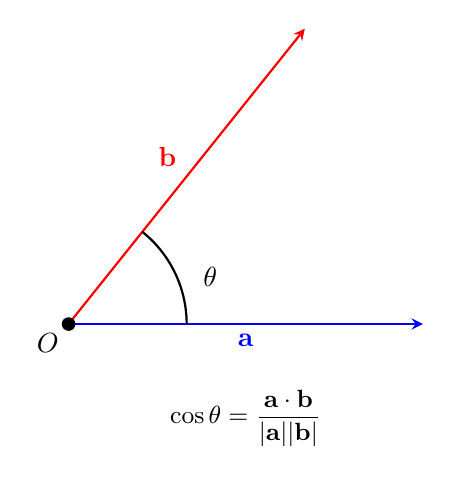
\begin{tikzpicture}[scale=1.5, >=stealth]
  % Two vectors with angle between them

  \draw[->, thick, blue] (0,0) -- (3, 0) node[midway, below] {$\mathbf{a}$};
  \draw[->, thick, red] (0,0) -- (2, 2.5) node[midway, above left] {$\mathbf{b}$};

  % Angle arc
  \draw[thick] (1, 0) arc (0:{atan2(2.5,2)}:1);
  \node at (1.2, 0.4) {$\theta$};

  % Formula
  \node[font=\small] at (1.5, -0.8) {$\cos\theta = \dfrac{\mathbf{a}\cdot\mathbf{b}}{|\mathbf{a}||\mathbf{b}|}$};

  % Origin
  \filldraw[black] (0,0) circle (1.5pt) node[below left] {$O$};
\end{tikzpicture}
\end{document}
